\documentclass[tikz,border=5pt]{standalone}
\usepackage[utf8]{inputenc}
\usepackage[T1]{fontenc}
\usepackage{lmodern,amsmath,amssymb}
\usepackage[american]{circuitikz}
\usepackage{pgfplots}
\pgfplotsset{compat=1.18}
\usetikzlibrary{circuits.logic.US,positioning,calc,arrows.meta,patterns,shapes.geometric}
\definecolor{Primary}{HTML}{1F77B4}
\begin{document}
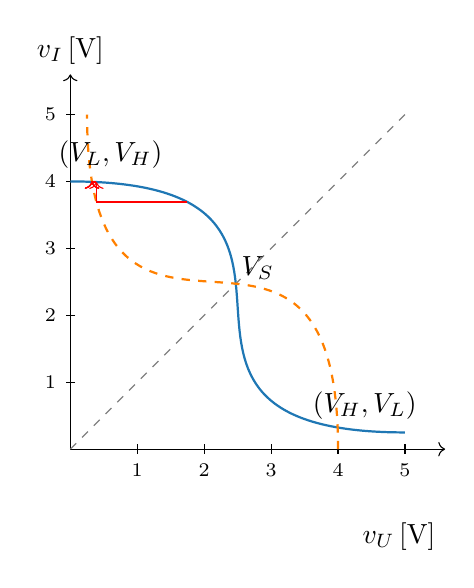
\begin{tikzpicture}[scale=.85]\draw[->] (0,0)--(5.6,0);\node[anchor=north east]at(5.6,-.95){$v_U\,[\mathrm V]$};\draw[->] (0,0)--(0,5.6) node[above]{$v_I\,[\mathrm V]$};\foreach \x in {1,...,5}{\draw (\x,.07)--(\x,-.07) node[below,font=\scriptsize]{\x};\draw (.07,\x)--(-.07,\x) node[left,font=\scriptsize]{\x};}\draw[Primary,thick] (0,4).. controls (4.75,4) and (.25,.25)..(5,.25);\draw[dashed,gray] (0,0)--(5,5);\draw[orange,thick,dashed] (4,0)..controls(4,4.75)and(.25,.25)..(.25,5);\draw[red,->] (1.75000,3.69203)--(0.38954,3.69203)--(0.38954,3.99076);\draw[red,->] (0.38954,3.99076)--(0.32443,3.99076)--(0.32443,3.99370);\draw[red,->] (0.32443,3.99370)--(0.32392,3.99370)--(0.32392,3.99372);\draw[red,->] (0.32392,3.99372)--(0.32392,3.99372)--(0.32392,3.99372);\draw[red,->] (0.32392,3.99372)--(0.32392,3.99372)--(0.32392,3.99372);\node at(.6,4.4){$(V_L,V_H)$};\node at(4.4,.65){$(V_H,V_L)$};\node at(2.8,2.7){$V_S$};\end{tikzpicture}
\end{document}
